\section{Design and Implementation}

\subsection{Subsystem Overview}
A lightweight Python framework was used to create an API, the communication bridge between Tiberius and the \gls{webinterface}. The \gls{webinterface} interacts with Tiberius by sending authenticated \gls{HTTP} \gls{POST} requests to the \gls{API} running on Tiberius' \gls{controlpi}.

Each request is sent with an X-Auth \gls{POST} parameter, with a authentication token. The authentication token set on Tiberius and the web server must match.

The \gls{API} and \gls{webinterface} server must be operating on the same network, to allow a route for packets to reach their destination address. In our instance we have used a \gls{VPN} to allow all devices to operate on the same network.

% Diagram illustrating all the modules used within the API and web interface.
\begin{figure}[!htb]
\begin{center}
\includegraphics[width=14cm]{api_modules.png}
\end{center}
\caption{API Modules}
\label{fig:api-modules}
\end{figure}

\begin{enumerate}[label=(\alph*)]
  \item Tiberius API: Uses Falcon to accept \gls{HTTP} \gls{POST} requests and act upon the body of the messages.  % (a)
  
  \item Sensors: Provides access to sensor data, bypassing the database.  (GPS, Ultrasonics, Compass) % (b)
  
  \item Task Control: Contains functions to start, pause and stop tasks. % (c)
  
  \item Database: Controlled access to database. Mostly query functions to allow web interface to fetch the latest sensor data. % (d)
  
  \item Debug: Immediately sends a response to every request received, used to test response rate. % (e)
  
  \item Motor Control: Allows Tiberius's motors to be controlled from anywhere on the network. % (f)
  
  \item Navigation: If a valid request is received, a point-to-point algorithm is started, navigating Tiberius to the given GPS waypoint. % (g)
  
  \item HTTP POST: All requests are of the POST variety, this is slightly more secure that GET requests, because parameters do not appear in the browser URL and no caching, history, or bookmarking can be done.% (h)
  
  \item Tiberius Web Server: Runs on an external web server, although it can be deployed on any PC if resources do not allow access to a web server. % (i)
  
  \item Control: Contains web pages with control panels, allowing the user to control the motors and robotic arm. % (j)
  \item Fleet: Lists all robots registered on the website. % (k)
  \item Mission Planner: Allows a user to design a mission by plotting waypoints and assigning tasks to those waypoints. % (l)
  \item Dashboard: The front page of the web application, provides links to other useful resources, and introduces the user to the purpose of the web application. % (m)
  \item Users: Manages the users that have access to the web application. % (n)
\end{enumerate}

\subsection{Control API}

% Diagram illustrating all the modules used within the API and web interface.
\begin{figure}[!htb]
\begin{center}
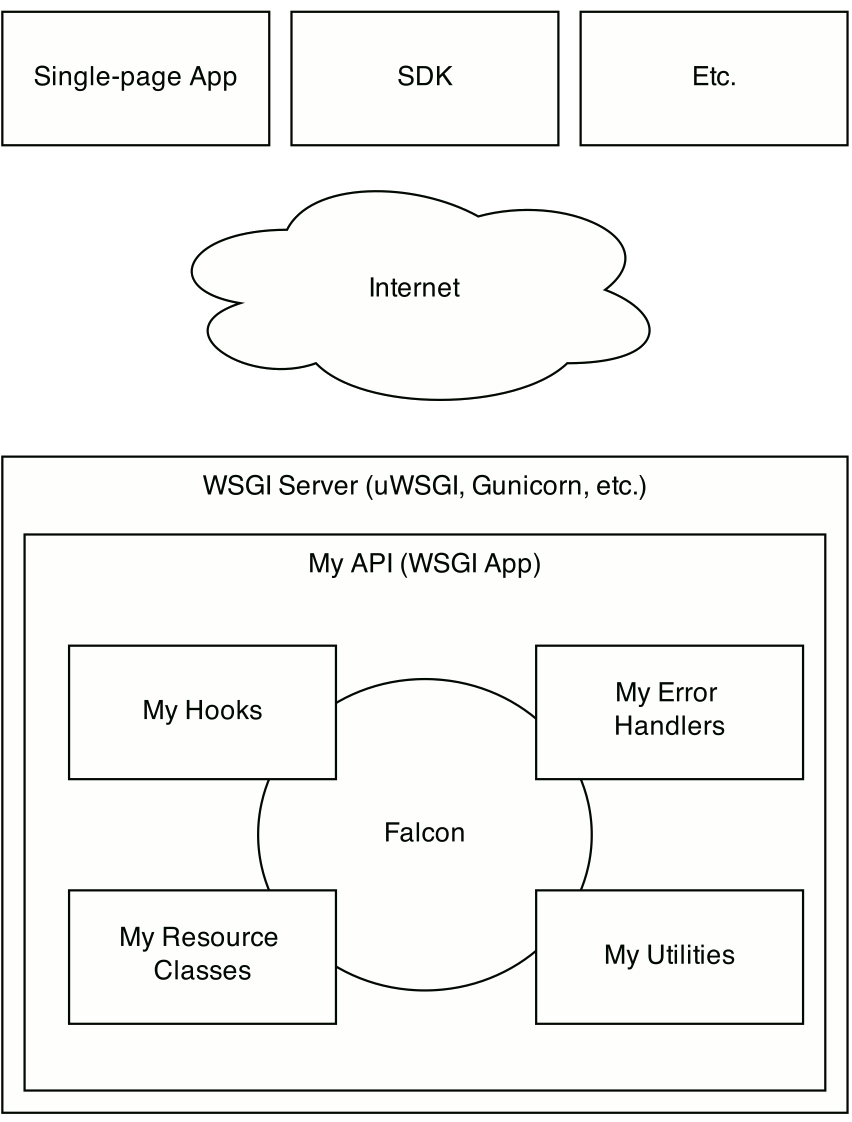
\includegraphics[width=12cm]{api_falcon.png}
\end{center}
\caption{Falcon Overview \cite{falcon-big-picture}}
\label{fig:api-falcon}
\end{figure}


\subsection{Web Interface}

\subsection{System Integration}